\chapter{Electric Current and Its Effects}\label{ch:g8:electric-current-effects}

The current has marched namelessly useful through five years of
circuits: lighting threads, spinning \omterm{ex:g6:circuits-and-safety:motor}{motors}, sounding \omterm{ex:g6:circuits-and-safety:motor}{buzzers}.
This year electricity turns quantitative --- meters, \omterm{def:g6:measurement-in-science:measuring}{units} and
laws --- and we open by taking inventory: what, exactly, can a
current \emph{do}? Three effects, it turns out, and the whole
electrical world is built from them.

\section{The three effects}

\begin{proposition}[The effects of the electric current]\label{prop:g8:electric-current-effects:three}
A current flowing through matter shows itself by three effects:
\begin{enumerate}
  \item the \emph{heating effect}\index{heating effect}: every
        current warms the \omterm{def:g4:conductors-insulators:conductor}{conductor} it crosses --- gently in good
        wires, fiercely in thin or overloaded ones, white-hot on
        purpose in filaments and toasters;
  \item the \emph{magnetic effect}\index{magnetic effect}: a
        current turns its surroundings magnetic --- a wire
        deflects a nearby \omterm{def:g4:magnets-and-compass:compass}{compass} needle, and a coiled wire
        becomes a true \omterm{def:g1:magnets:magnet}{magnet} with poles, switchable at will;
  \item the \emph{chemical effect}\index{chemical effect}:
        crossing certain \omterm{def:g3:solids-liquids-gases:liquid}{liquids}, a current drives chemical
        change --- splitting water into two gases, plating
        spoons with silver, charging and discharging every
        \omterm{def:g3:first-electric-circuit:battery}{battery}.
\end{enumerate}
\end{proposition}

\begin{example}[The heating effect at work]\label{ex:g8:electric-current-effects:heating}
Deliberate: the toaster's glowing bars, the kettle's hidden
coil, the old lamp's white-hot filament, the \omterm{def:g7:short-circuits-safety:fuse}{fuse} built to \omterm{def:g2:ice-water-steam:meltfreeze}{melt}
first. Unwanted: warm phone chargers, hot laptop undersides ---
and the \omterm{def:g7:short-circuits-safety:device}{short circuit}'s menace, which you studied as the
villain's signature. One effect, servant and danger, dosed by
how hard the current runs --- a dose we learn to \emph{\omterm{def:g6:measurement-in-science:measuring}{measure}}
in the next chapter.
\end{example}

\begin{omfigure}
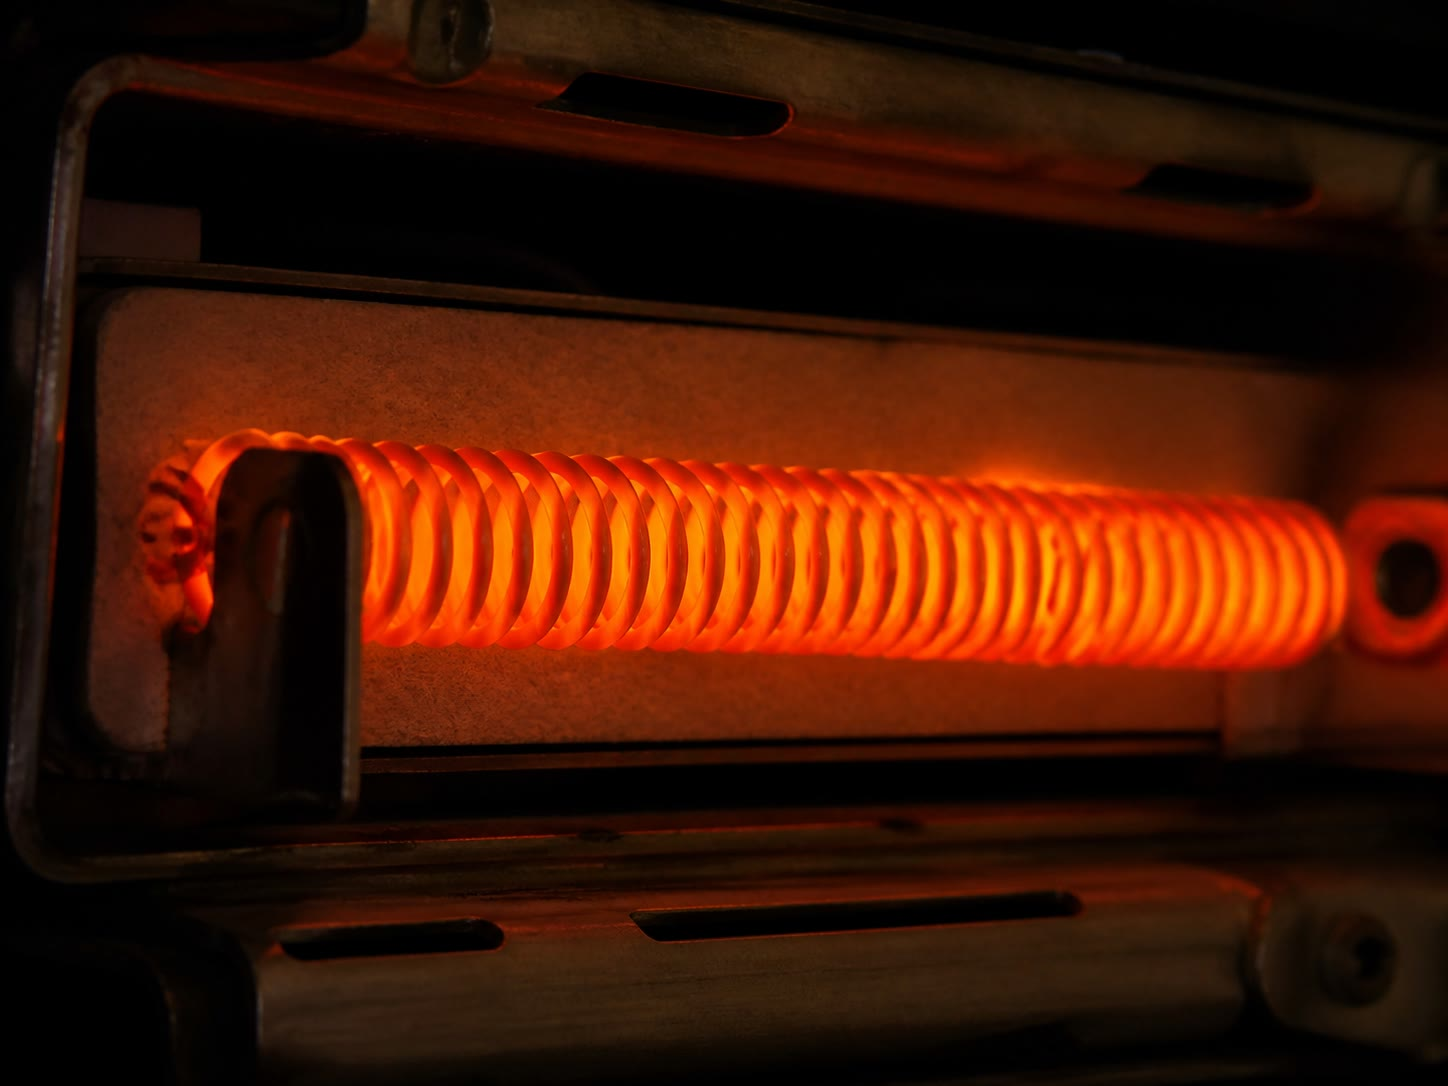
\includegraphics[width=0.5\linewidth]{images/book1/ai/g8-current-heating-coil.jpg}

{\small The thermal effect, glowing: current forced through the toaster's resistive coil \omterm{def:g5:heat-and-insulation:heat}{heats} it red-hot.}
\end{omfigure}

\section{The current makes magnets}

\begin{example}[The compass betrays the wire]\label{ex:g8:electric-current-effects:oersted}
Two centuries ago, during a lecture, a physicist noticed a
\omterm{def:g4:magnets-and-compass:compass}{compass} needle twitch each time he closed a circuit on the
bench beside it. That twitch --- barely a trembling of a needle
--- was the first bridge ever seen between electricity and
magnetism, two sciences until then as separate as weather and
music. Lay a \omterm{def:g4:magnets-and-compass:compass}{compass} beside a wire and switch on: the needle
swings aside; reverse the current, and it swings the other way.
The current creates magnetism around itself, with a direction.
\end{example}

\begin{definition}[Electromagnet]\label{def:g8:electric-current-effects:electromagnet}
An \emph{electromagnet}\index{electromagnet} is a coil of
insulated wire --- often wound on an iron core --- that becomes
a \omterm{def:g1:magnets:magnet}{magnet} while current flows through it: \omterm{def:g4:magnets-and-compass:poles}{north pole}, \omterm{def:g4:magnets-and-compass:poles}{south
pole}, iron-grabbing power and all. Unlike any stone \omterm{def:g1:magnets:magnet}{magnet}, it
obeys a \omterm{ex:g3:first-electric-circuit:switch}{switch}: current on, \omterm{def:g1:magnets:magnet}{magnet} on; current off, \omterm{def:g1:magnets:magnet}{magnet}
gone; current reversed, poles exchanged.
\end{definition}

\begin{omfigure}
\begin{tikzpicture}[scale=0.85]
  \draw[thick, fill=omExo, fill opacity=0.3]
    (1.2,1.0) rectangle (5.4,1.9);
  \foreach \x in {1.5,2.1,...,5.1} {
    \draw[very thick, omDef] (\x,0.82) arc (200:340:0.35 and 0.5);
  }
  \draw[thick, omDef] (1.3,0.95) -- (0.4,0.4);
  \draw[thick, omDef] (5.3,0.95) -- (6.2,0.4);
  \node[below, font=\small] at (0.5,0.3) {to the battery};
  \node[above, font=\small] at (3.3,2.05) {iron core in a coil};
  \draw[thick] (7.4,1.05) ellipse (0.32 and 0.14);
  \draw[thick] (8.15,1.3) ellipse (0.32 and 0.14);
  \draw[thick] (7.5,1.6) ellipse (0.32 and 0.14);
  \node[right, font=\small] at (8.7,1.3)
    {paperclips: held while the switch is closed};
\end{tikzpicture}

{\small The \omterm{def:g8:electric-current-effects:electromagnet}{electromagnet}: a coil and a current make a \omterm{def:g1:magnets:magnet}{magnet}
that a \omterm{ex:g3:first-electric-circuit:switch}{switch} can create, destroy, or flip.}
\end{omfigure}

\begin{example}[Switchable magnetism runs the world]\label{ex:g8:electric-current-effects:uses}
The scrapyard crane grips a car with an \omterm{def:g8:electric-current-effects:electromagnet}{electromagnet} and drops
it by opening a \omterm{ex:g3:first-electric-circuit:switch}{switch} --- try that with a stone \omterm{def:g1:magnets:magnet}{magnet}.
Electric door-locks, the clack of a relay, the doorbell's
hammer (an \omterm{def:g8:electric-current-effects:electromagnet}{electromagnet} snatching it against the bell, cutting
its own current, springing back: rattle made law), the reading
head of old telephones, and --- supremely --- every electric
\omterm{ex:g6:circuits-and-safety:motor}{motor}: current-made magnetism pushing against \omterm{def:g1:magnets:magnet}{magnets}, thousands
of times a second. The \omterm{prop:g8:electric-current-effects:three}{magnetic effect} is the muscle of the
electrical age.
\end{example}

\begin{method}[Winding an electromagnet]\label{met:g8:electric-current-effects:wind}
\begin{enumerate}
  \item \omterm{def:g2:air-around-us:wind}{wind} a \omterm{def:g2:measuring-length:units}{metre} or two of thin insulated wire in tight,
        tidy turns around a large iron nail or bolt, leaving two
        free ends;
  \item connect the ends to a \omterm{def:g3:first-electric-circuit:battery}{battery} through a \omterm{ex:g3:first-electric-circuit:switch}{switch} (never
        directly for long --- the coil is nearly a \omterm{def:g7:short-circuits-safety:device}{short
        circuit} and warms: the \omterm{prop:g8:electric-current-effects:three}{heating effect} chaperones the
        experiment);
  \item close the \omterm{ex:g3:first-electric-circuit:switch}{switch} briefly: the nail-head grabs
        paperclips; open it: they drop;
  \item test with a \omterm{def:g4:magnets-and-compass:compass}{compass}: the coil's two ends behave as N and
        S poles --- and swap when you reverse the \omterm{def:g3:first-electric-circuit:battery}{battery}.
\end{enumerate}
More turns, stronger grip: dose the magnetism by winding.
\end{method}

\section{The chemical effect}

\begin{example}[Current through water]\label{ex:g8:electric-current-effects:electrolysis}
Dip two pencil-lead electrodes wired to a \omterm{def:g3:first-electric-circuit:battery}{battery} into water
made slightly conducting (a spoon of washing soda helps), and
watch: tiny bubbles stream from both leads --- two different
gases, born of the water itself, twice the \omterm{def:g6:mass-and-volume:volume}{volume} at one lead
as at the other. The current is dismantling water into its two
invisible components. This door between electricity and
chemistry --- \emph{electrolysis} --- plates cheap spoons with
silver, wins aluminium from ore, and belongs mostly to your
chemistry course; physics salutes it and moves on.
\end{example}

\begin{example}[Every battery is the effect run backward]\label{ex:g8:electric-current-effects:battery}
Inside every \omterm{def:g3:first-electric-circuit:battery}{battery}, chemistry pushes the current: stored
chemical \omterm{def:g5:everyday-energy:energy}{energy} drives the march, spending itself as it serves
--- the emptying you have known since the flashlight dimmed.
Rechargeable cells close the circle: the charger \omterm{def:g2:pushes-and-pulls:force}{forces} current
through \emph{backward}, and the \omterm{prop:g8:electric-current-effects:three}{chemical effect} rebuilds the
store. Chemical to electrical, electrical to chemical: one
effect, both directions, the whole \omterm{def:g3:first-electric-circuit:battery}{battery} industry.
\end{example}

\begin{remark}[Effects as detectors]\label{rem:g8:electric-current-effects:detect}
The three effects answer a question that stumped you as the
tester's apprentice: how do you \emph{see} a current --- an
invisible march in an \omterm{def:g7:light-sources-propagation:coats}{opaque} wire? By its deeds. A warming
wire, a twitching \omterm{def:g4:magnets-and-compass:compass}{compass}, a streaming bubble: each betrays the
march. Every current-measuring instrument ever built reads one
of the three effects --- and the one waiting in the next
chapter reads the magnetic twitch, refined into a numbered
dial.
\end{remark}

\section{Exercises}

\begin{exercise}[$\star$]\label{exo:g8:electric-current-effects:1}
Name the three effects of the \omterm{def:g7:circuits-series-parallel:current}{electric current}, each with one
servant use.
\end{exercise}

\begin{exercise}[$\star$]\label{exo:g8:electric-current-effects:2}
Which effect, in each scene: a \omterm{def:g7:short-circuits-safety:fuse}{fuse} \omterm{def:g6:water-states:changes}{melting}; \ a doorbell
hammering; \ bubbles at the pencil leads; \ a toaster's glow;
\ a scrapyard crane's grip?
\end{exercise}

\begin{exercise}[$\star$]\label{exo:g8:electric-current-effects:3}
What did the twitching \omterm{def:g4:magnets-and-compass:compass}{compass} beside the lecture bench reveal?
What happens to the twitch when the current reverses?
\end{exercise}

\begin{exercise}[$\star$]\label{exo:g8:electric-current-effects:4}
Give three powers an \omterm{def:g8:electric-current-effects:electromagnet}{electromagnet} has that no stone \omterm{def:g1:magnets:magnet}{magnet} can
match.
\end{exercise}

\begin{exercise}[$\star$]\label{exo:g8:electric-current-effects:5}
In the winding method, why must the wire be insulated? And why
must the coil not stay connected long without a working load?
\end{exercise}

\begin{exercise}[$\star$]\label{exo:g8:electric-current-effects:6}
How does the crane operator release the car? Contrast with what
a stone \omterm{def:g1:magnets:magnet}{magnet} of equal strength would demand.
\end{exercise}

\begin{exercise}[$\star$]\label{exo:g8:electric-current-effects:7}
What \omterm{def:g5:everyday-energy:energy}{energy} conversion happens inside a \omterm{def:g3:first-electric-circuit:battery}{battery} in use? And
inside a rechargeable \omterm{def:g3:first-electric-circuit:battery}{battery} on its charger?
\end{exercise}

\begin{exercise}[$\star$]\label{exo:g8:electric-current-effects:8}
Why are the three effects precious as \emph{detectors}? Which
effect will the next chapter's instrument refine into a
number?
\end{exercise}

\begin{exercise}[$\star\star$]\label{exo:g8:electric-current-effects:9}
The doorbell: an \omterm{def:g8:electric-current-effects:electromagnet}{electromagnet} snatches the hammer toward the
bell, but the moving hammer breaks its own circuit; a spring
returns it, remaking the contact --- and so on. Walk through
one full cycle and explain why the design \emph{must} rattle
rather than hold.
\end{exercise}

\begin{exercise}[$\star\star$]\label{exo:g8:electric-current-effects:10}
A relay is a \omterm{ex:g3:first-electric-circuit:switch}{switch} closed by an \omterm{def:g8:electric-current-effects:electromagnet}{electromagnet}: a small current
in the coil closes contacts that carry a big current in another
circuit. Explain why this lets a delicate thermostat safely
command a hungry electric heater --- and which two circuits
never touch.
\end{exercise}

\begin{exercise}[$\star\star$]\label{exo:g8:electric-current-effects:11}
Your \omterm{def:g4:magnets-and-compass:compass}{compass} needle twitches whenever a hidden wire in the wall
carries current. Design a wall-wire finder from this fact:
protocol, what a strong twitch means, and one honest limit of
the instrument (think of what else moves \omterm{def:g4:magnets-and-compass:compass}{compass} needles).
\end{exercise}

\begin{exercise}[$\star\star\star$]\label{exo:g8:electric-current-effects:12}
An electric \omterm{ex:g6:circuits-and-safety:motor}{motor}, in outline: a coil on an axle sits between
the poles of a \omterm{def:g1:magnets:magnet}{magnet}; current makes the coil a \omterm{def:g1:magnets:magnet}{magnet}; the
push-and-pull of poles turns the axle --- and just as the coil
would settle aligned, the current through it is reversed, so it
must chase alignment forever. Explain, pole by pole, why the
reversal is indispensable --- what would the \omterm{ex:g6:circuits-and-safety:motor}{motor} do without
it? (You have just explained why \omterm{ex:g6:circuits-and-safety:motor}{motors} contain a reversing
contact --- and half of how the electrical age turns its
wheels.)
\end{exercise}

\section{Problem: The Inventor's Workshop}

\begin{problem}[{Weekend problem --- one battery, three effects,
five inventions; an evening in the inventor's
workshop}]\label{pb:g8:electric-current-effects:1}
The workshop bench holds batteries, wire, iron nails, a
\omterm{def:g4:magnets-and-compass:compass}{compass}, two pencil leads, a jar of soda water --- and a
notebook of half-built inventions to assess.

\medskip\noindent\textbf{Part I --- Taking inventory.}
\begin{enumerate}
  \item Sketch the workshop's three-effect test bench: for one
        \omterm{def:g3:first-electric-circuit:battery}{battery} and a \omterm{ex:g3:first-electric-circuit:switch}{switch}, describe a setup that shows all
        three effects at once (a thin wire to warm, a \omterm{def:g4:magnets-and-compass:compass}{compass}
        beside a lead, the jar in the loop). In what
        arrangement must the three demonstrations sit ---
        series or parallel --- for one \omterm{ex:g3:first-electric-circuit:switch}{switch} to run them all?
  \item The thin demonstration wire grows warm but the thick
        supply wires stay cool, in the same loop. Which
        chapter-one fact about the series loop makes this
        \emph{more} interesting than it looks --- what is equal
        in both wires, and what differs?
  \item The \omterm{def:g4:magnets-and-compass:compass}{compass} twitches east when the \omterm{ex:g3:first-electric-circuit:switch}{switch} closes. What
        two changes, made together, would leave the twitch
        exactly as it was?
  \item Bubbles stream twice as fast from one pencil lead as
        the other. What does this hint about water's two
        components? (Chemistry will confirm the ratio.)
\end{enumerate}

\medskip\noindent\textbf{Part II --- Assessing the inventions.}
\begin{enumerate}[resume]
  \item Invention: ``the silent doorbell'' --- an \omterm{def:g8:electric-current-effects:electromagnet}{electromagnet}
        that pulls a soft felt hammer once and holds it until
        the button is released. Which piece of the classic
        doorbell's mechanism must the inventor \emph{remove},
        and what will the visitor hear?
  \item Invention: ``the magnetic sorter'' --- scrap on a
        conveyor passes under an \omterm{def:g8:electric-current-effects:electromagnet}{electromagnet} that lifts out
        iron and steel. What happens at the drop bin, and why
        does the sorter leave aluminium cans on the belt
        (two \omterm{def:g1:magnets:magnet}{magnet} facts from earlier years answer)?
  \item Invention: ``the pole-flipper'' --- a \omterm{def:g4:magnets-and-compass:compass}{compass} mounted
        over a coil, flipping each time a hidden \omterm{ex:g3:first-electric-circuit:switch}{switch}
        reverses the \omterm{def:g3:first-electric-circuit:battery}{battery}. Which property of
        current-made magnetism is being exploited?
  \item Invention: ``the eternal electroplater'' --- silver
        plating powered by a \omterm{def:g3:first-electric-circuit:battery}{battery} that ``recharges itself
        from the plating''. Veto it, citing the chapter's two
        \omterm{def:g3:first-electric-circuit:battery}{battery} directions and an older law about \omterm{def:g5:everyday-energy:energy}{energy}.
\end{enumerate}

\medskip\noindent\textbf{Part III --- The night's masterpiece.}
The inventor closes with a crane game for the fair: a joystick,
a small \omterm{def:g8:electric-current-effects:electromagnet}{electromagnet} on strings, a bin of iron trinkets.
\begin{enumerate}[resume]
  \item Script the winning move in effect-language: what
        happens at ``grab'', during the swing, and at
        ``release''?
  \item Fairgoers complain the crane drops prizes mid-swing
        whenever the old \omterm{def:g3:first-electric-circuit:battery}{battery} sags. Which property of the
        \omterm{def:g8:electric-current-effects:electromagnet}{electromagnet} --- virtue and weakness in one --- is on
        display?
  \item The inventor doubles the coil's turns to help. Predict
        the effect on grip, and name the other dose (from the
        \omterm{def:g3:first-electric-circuit:battery}{battery} side) that next chapter will let us number.
  \item Notebook's last page: write the workshop's summary ---
        one sentence per effect, each naming its finest servant
        invention of the evening.
\end{enumerate}
\end{problem}
